\section{Organizacion de RRHH}

A continuación se van a enumerar los roles que van a tener los miembros del equipo de desarrollo, estos roles cubren todas las áreas de conocimiento que son necesarias para el correcto avance del proyecto. Estos son:
\begin{itemize}
    \item Requerimientos: El cual se encarga de mantener el análisis y la gestión de los requeimientos del proyecto
    \item Diseño: El cual se encarga de utilizar el conocimiento sobre el dominio del problema para reducier el nivel de abstracción de los requerimientos al generar la estructura especifica del sistema
    \item Implementación: Se encargará de llevar a cabo los cambios mencionados
    \item Aseguramiento de calidad: Se encargará de realizar las pruebas de código y de realizar el análisis de la calidad del código, los casos de pruebas y los requeimientos
\end{itemize}

\begin{figure}[H]
    \centering
    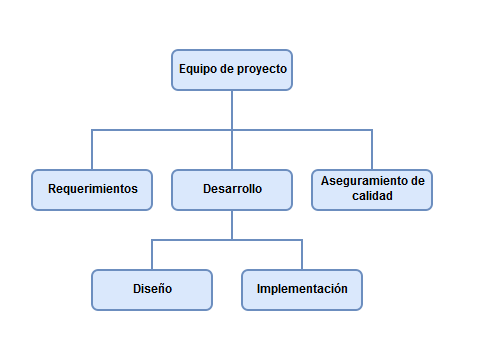
\includegraphics[scale=0.6]{Files/OBS.png}
    \caption{Estructura de desglose de la organización}
    \label{fig:clases}
\end{figure}

A continuación de detallarán los integrantes del equipo de proyecto:

\prettyTable{|l|l|l|l|l|}{
    \textbf{Nombre} & \textbf{Frecuencia} & \textbf{Comienza} & \textbf{Finaliza} \\ \hline
    Marcelo Plada & - & Fecha inicio proceso & Fecha entrega \\ \hline
    Vincent Silva & - & Fecha inicio proceso & Fecha entraga \\ \hline
}

Los roles que se van a asumir estarán repartidos de la siguiente manera:

\prettyTable{|l|c|c|}{
    \textbf{Rol} & \textbf{\mlcell{Vincent Silva}} & \textbf{\mlcell{Marcelo plada}} \\ \hline
    Requerimientos & R & C \\ \hline
    Diseño & R & C \\ \hline
    Implementación & C & R \\ \hline
    Aseguramiento de calidad & C & R \\ \hline
}

Donde cada rol podrá tener un consultado que tomará parte en las tareas pero para cada tipo de tarea habrá un responsable el cual se encargará de realizar la división de tareas en esa área. Al ser un grupo reducido cada uno de los integrántes será responsable de mas de una tarea y deberá ser consultante en el resto.

\begin{comment}

Describir roles y responsabilidades basado en OBS.
Incluir un organigrama del proyecto.
Máximo: 1 página.

Se puede incluir una lista con los nombres de los integrantes del proyecto y sus roles, por ej:

Roles y Responsabilidades: rol + autoridad + responsabilidad + competencias.

Organigrama: del personal del Proyecto

Plan para la gestión de personal: Adquisición de personal + Calendarios de recursos + Plan de liberación del personal + Necesidades de capacitación + Reconocimiento y recompensas + Cumplimiento + Seguridad.
\end{comment}